%%%%%%%%%%%%%%%%%%%%%%%%%%%%%%%%%%%%%%%%%%%%%%%%%%%%%%%%%%%%%%%%%%%%%%%%%%%
%
% Template for a LaTex article in English.
%
%%%%%%%%%%%%%%%%%%%%%%%%%%%%%%%%%%%%%%%%%%%%%%%%%%%%%%%%%%%%%%%%%%%%%%%%%%%

\documentclass[a4, 12px]{article}

% AMS packages:
\usepackage{amsmath, amsthm, amsfonts, graphicx, subfigure, enumitem}
\usepackage[bahasai]{babel}

% Theorems
%-----------------------------------------------------------------
\newtheorem{thm}{Theorem}[section]
\newtheorem{cor}[thm]{Corollary}
\newtheorem{lem}[thm]{Lemma}
\newtheorem{prop}[thm]{Proposition}
\theoremstyle{definition}
\newtheorem{defn}[thm]{Definition}
\theoremstyle{remark}
\newtheorem{rem}[thm]{Remark}

% Shortcuts.
% One can define new commands to shorten frequently used
% constructions. As an example, this defines the R and Z used
% for the real and integer numbers.
%-----------------------------------------------------------------
\def\RR{\mathbb{R}}
\def\ZZ{\mathbb{Z}}

% Similarly, one can define commands that take arguments. In this
% example we define a command for the absolute value.
% -----------------------------------------------------------------
\newcommand{\abs}[1]{\left\vert#1\right\vert}

% Operators
% New operators must defined as such to have them typeset
% correctly. As an example we define the Jacobian:
% -----------------------------------------------------------------
\DeclareMathOperator{\Jac}{Jac}

%-----------------------------------------------------------------
\title{Eksplorasi Hyperparameter CNN dan Neural Network}
\author{Imam Ekowicaksono -
  \small (NIM. 33220306)
  %\small E12345\\
  %\small Spain
}
\date{}

\begin{document}
\maketitle

%\abstract{This is a simple template for an article written in \LaTeX.}

\section{Pendahuluan}

Persoalan klasifikasi merupakan salah satu persoalan populer yang ada pada topik pembelajaran mesin (\textit{machine learning}). Persoalan klasifikasi ini dapat ditangani dengan menggunakan metode klasifikasi yang berbasis neural network dengan mengklasifikasi data gambar Fashion MNIST. 

\section{Klasifikasi}\label{sec:klasifikasi}

Persoalan klasifikasi ini menggunakan dataset Fashion MNIST untuk dilakukan training dan testing. Fashion-MNIST adalah kumpulan data gambar traning sebanyak 60.000 sampel dan testing sebanyak 10.000 sampel. Setiap sampel terdiri dari gambar grayscale berukuran 28x28 dan memiliki 10 kelas label.

Pada persoalan klasifikasi ini, dilakukan perancangan model CNN dengan menggunakan keras. Keras adalah library untuk membuat model CNN. Keras memiliki beberapa library yang bisa digunakan untuk membuat model CNN. Model terbaik yang dapat diselesaikan sampai dengan saat ini menggunakan 2 convolutional layer dan 2 fully connected layer.

Percobaan dilakukan dengan mengembangkan prebuild model handwritten digit recognition model yang sudah ada. Percobaan pertama dilakukan dengan mengecek ukuran kernel yang optimal untuk menghasilkan model CNN yang optimal. Hasil yang optimal diperoleh dengan menggunakan kernel berukuran $3\times 3$. Hasil eksplorasi disajikan pada gambar \ref{fig:k1} berikut:

% TODO: \usepackage{graphicx} required
\begin{figure}[!h]
	\centering
	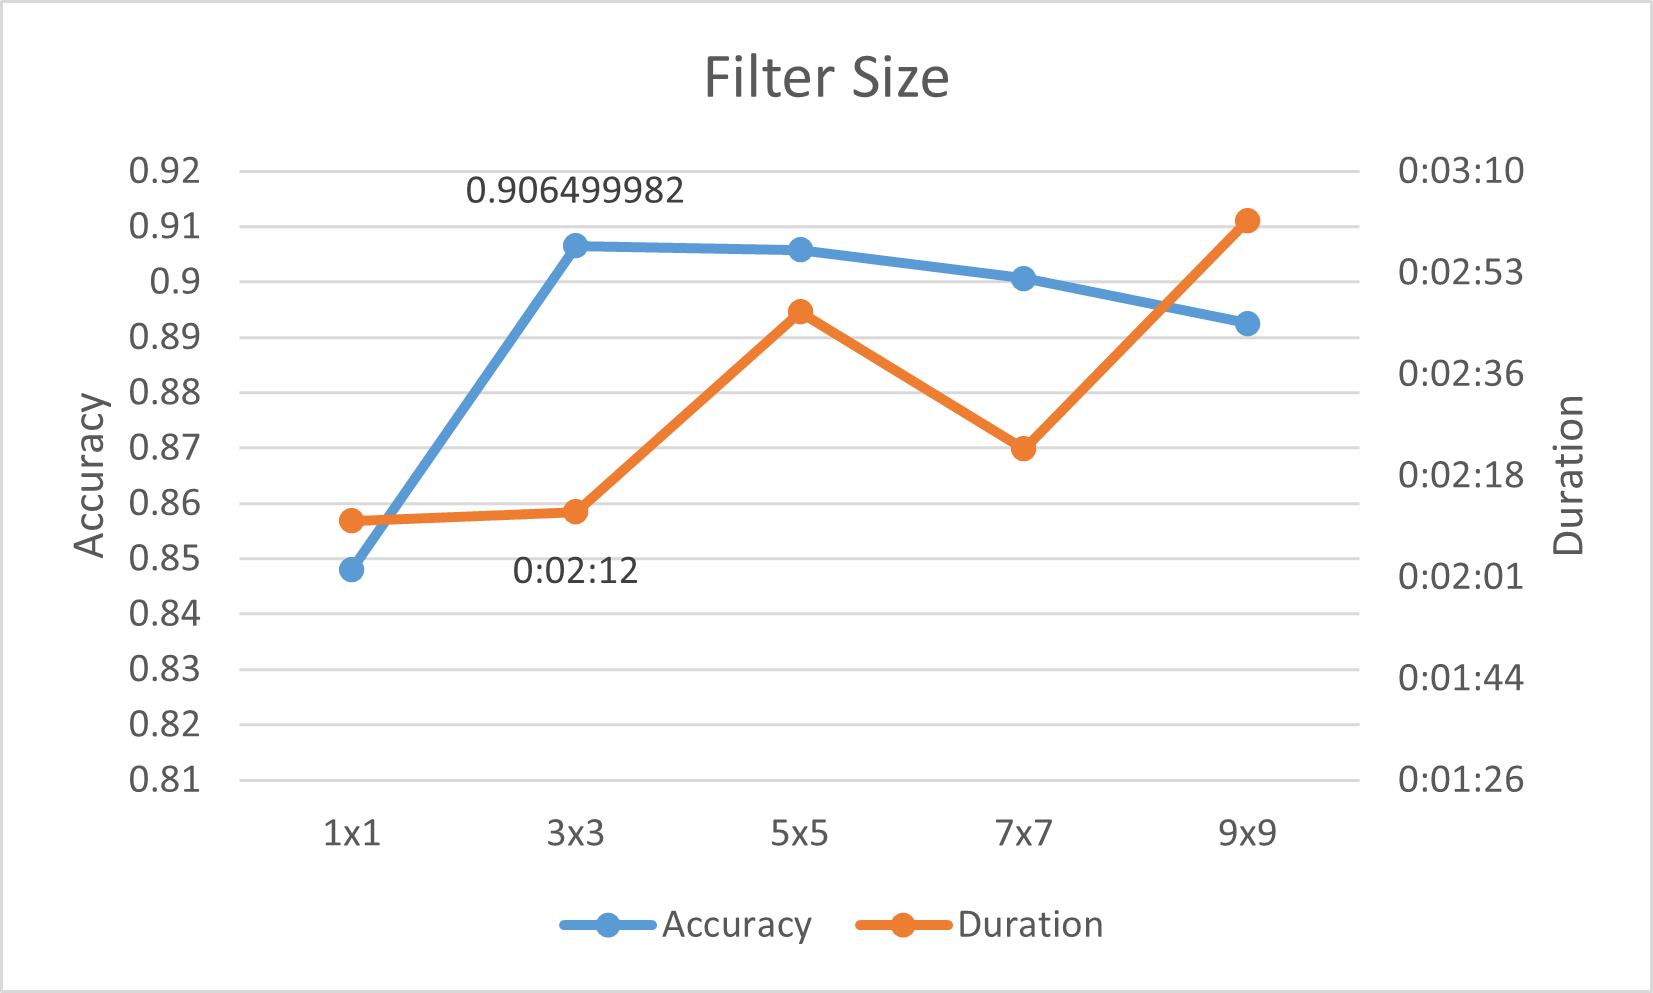
\includegraphics[width=0.45\linewidth]{src/K1}
	\caption{Akurasi berdasarkan ukuran kernel}
	\label{fig:k1}
\end{figure}

Setelah mendapatkan ukuran kernel yang optimal, langkah berikutnya adalah mengecek jumlah convolutional layer yang optimal. Percobaan pertama dilakukan dengan menggunakan 2 convolutional layer. Percobaan berikutnya dilakukan dengan 3 convolutional layer sampai dengan 5 convolutional layer. Hasil eksplorasi disajikan pada gambar \ref{fig:k2} berikut:

% TODO: \usepackage{graphicx} required
\begin{figure}[!h]
	\centering
	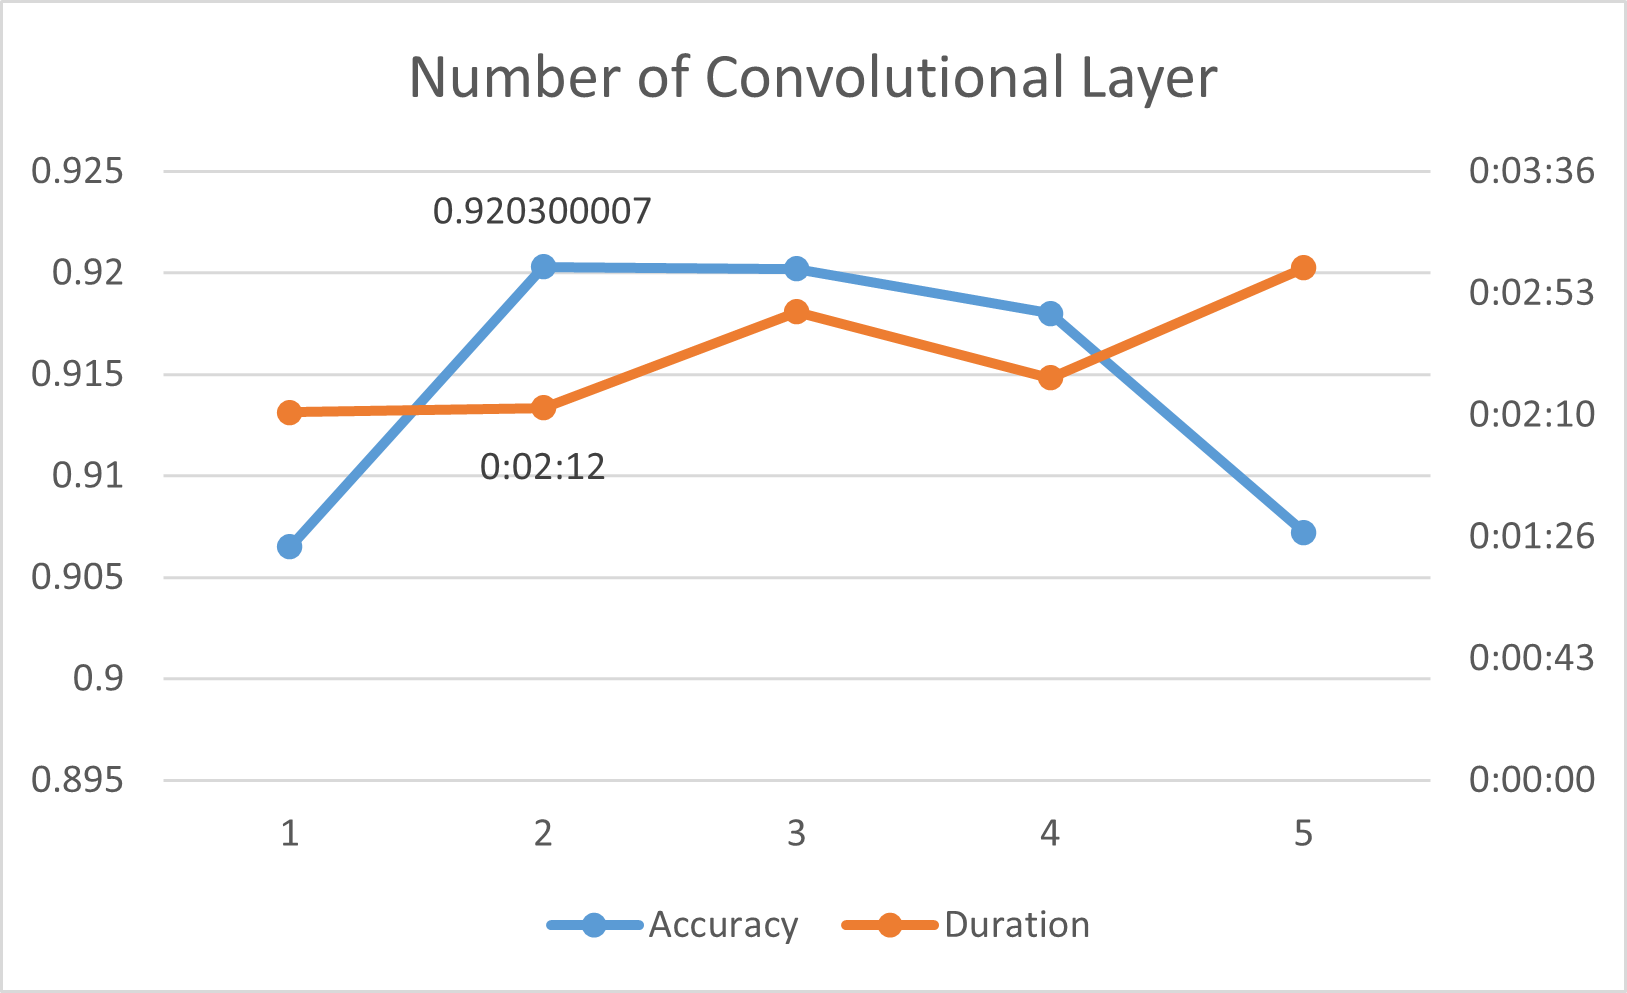
\includegraphics[width=0.7\linewidth]{src/K2}
	\caption{Akurasi berdasarkan jumlah convolutional layer}
	\label{fig:k2}
\end{figure}

Pada percobaan kedua ini diperoler jumlah convolutional layer yang optimal adalah 2 convolutional layer dengan akurasi sebesar 90.65\%.

Percobaan berikutnya adalah mengecek jumlah kernel pada setiap convolutional layer yang optimal. Percobaan dilakukan dengan mengkombinasi seluruh kemungkinan jumlah kernel pada setiap convolutional layer. Hasil eksplorasi disajikan pada gambar \ref{fig:k3} berikut:

% TODO: \usepackage{graphicx} required
\begin{figure}[!h]
	\centering
	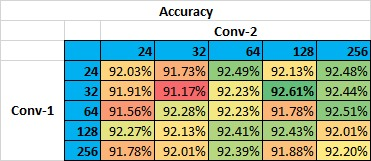
\includegraphics[width=0.7\linewidth]{src/K3}
	\caption{Akurasi dari setiap kemungkinan jumlah kernel pada setiap convolutional layer}
	\label{fig:k3}
\end{figure}

Percobaan ini menghasilkan akurasi terbaik pada 92.61\% dengan jumlah kernel sebesar 32 pada convolutional layer pertama dan 128 kernel pada convolutional layer kedua.

Percebaan berikutnya adalah mengecek jumlah dense layer yang optimal. Percobaan pertama dilakukan dengan menggunakan 2 dense layer. Percobaan berikutnya dilakukan dengan 3 dense layer sampai dengan 5 dense layer. Hasil eksplorasi disajikan pada gambar \ref{fig:k4} berikut:

% TODO: \usepackage{graphicx} required
\begin{figure}[!h]
	\centering
	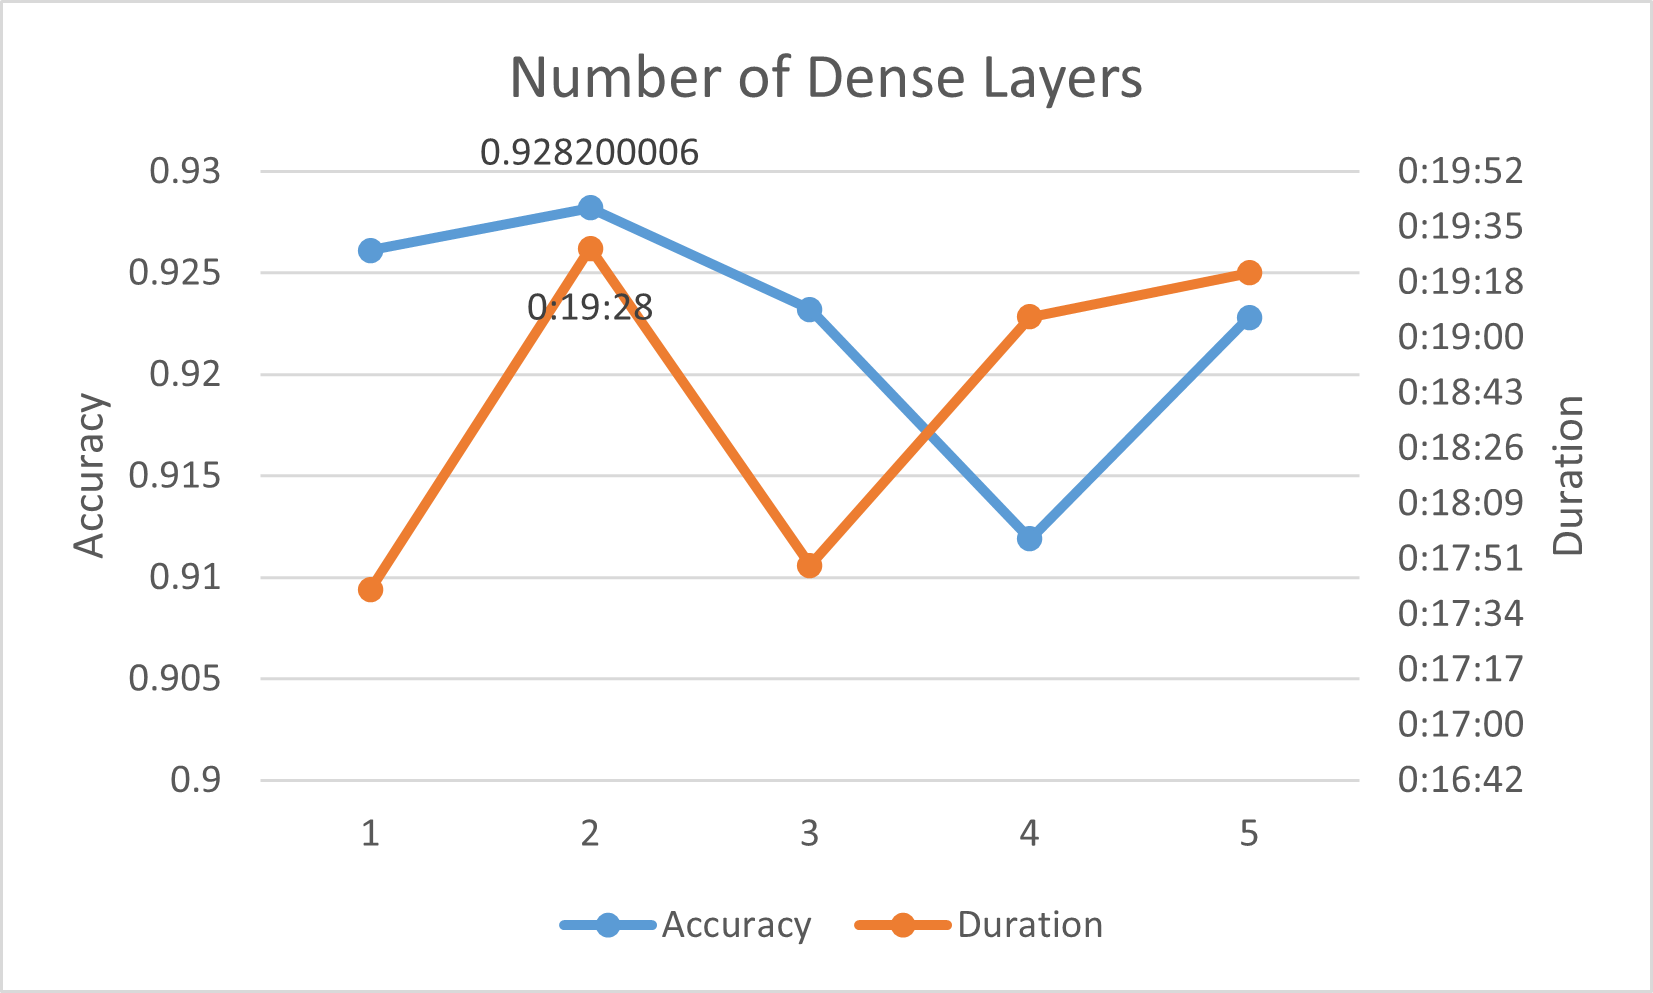
\includegraphics[width=0.7\linewidth]{src/K4}
	\caption{Akurasi dari setiap kemungkinan jumlah dense layer}
	\label{fig:k4}
\end{figure}

Percobaan ini menghasilkan jumlah dense layer yang optimal sebanyak 2 dense layer dengan akurasi mencapai 92.82\%.

Percobaan berikutnya adalah mengecek jumlah neuron pada setiap dense layer yang optimal. Percobaan pertama dilakukan dengan menggunakan 24 neuron pada setiap dense layer. Percobaan berikutnya dilakukan dengan 32 neuron pada setiap dense layer (dengan kelipatan 2) sampai dengan 256 neuron pada setiap dense layer. Hasil eksplorasi disajikan pada gambar \ref{fig:k5} berikut:

% TODO: \usepackage{graphicx} required
\begin{figure}[!h]
	\centering
	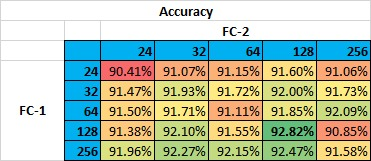
\includegraphics[width=0.7\linewidth]{src/K5}
	\caption{Akurasi dari setiap kemungkinan jumlah neuron pada setiap Dense Layer}
	\label{fig:k5}
\end{figure}

Dari percobaan tersebut, diperoleh akurasi mencapai 92.82\% dengan jumlah neuron pada setiap dense layer sebanyak 128 neuron.
Percobaan berikutnya adalah mengecek jenis optimizer yang disediakan oleh keras yang memberikan akurasi terbaik. Beberapa optimizer seperti Adam, SGD, RMSprop, Adagrad, Adadelta, Adamax, Nadam, TFOptimizer, dan FtrlOptimizer telah dieksplorasi. Hasil eksplorasi disajikan pada gambar \ref{fig:k6} berikut:

% TODO: \usepackage{graphicx} required
\begin{figure}[!h]
	\centering
	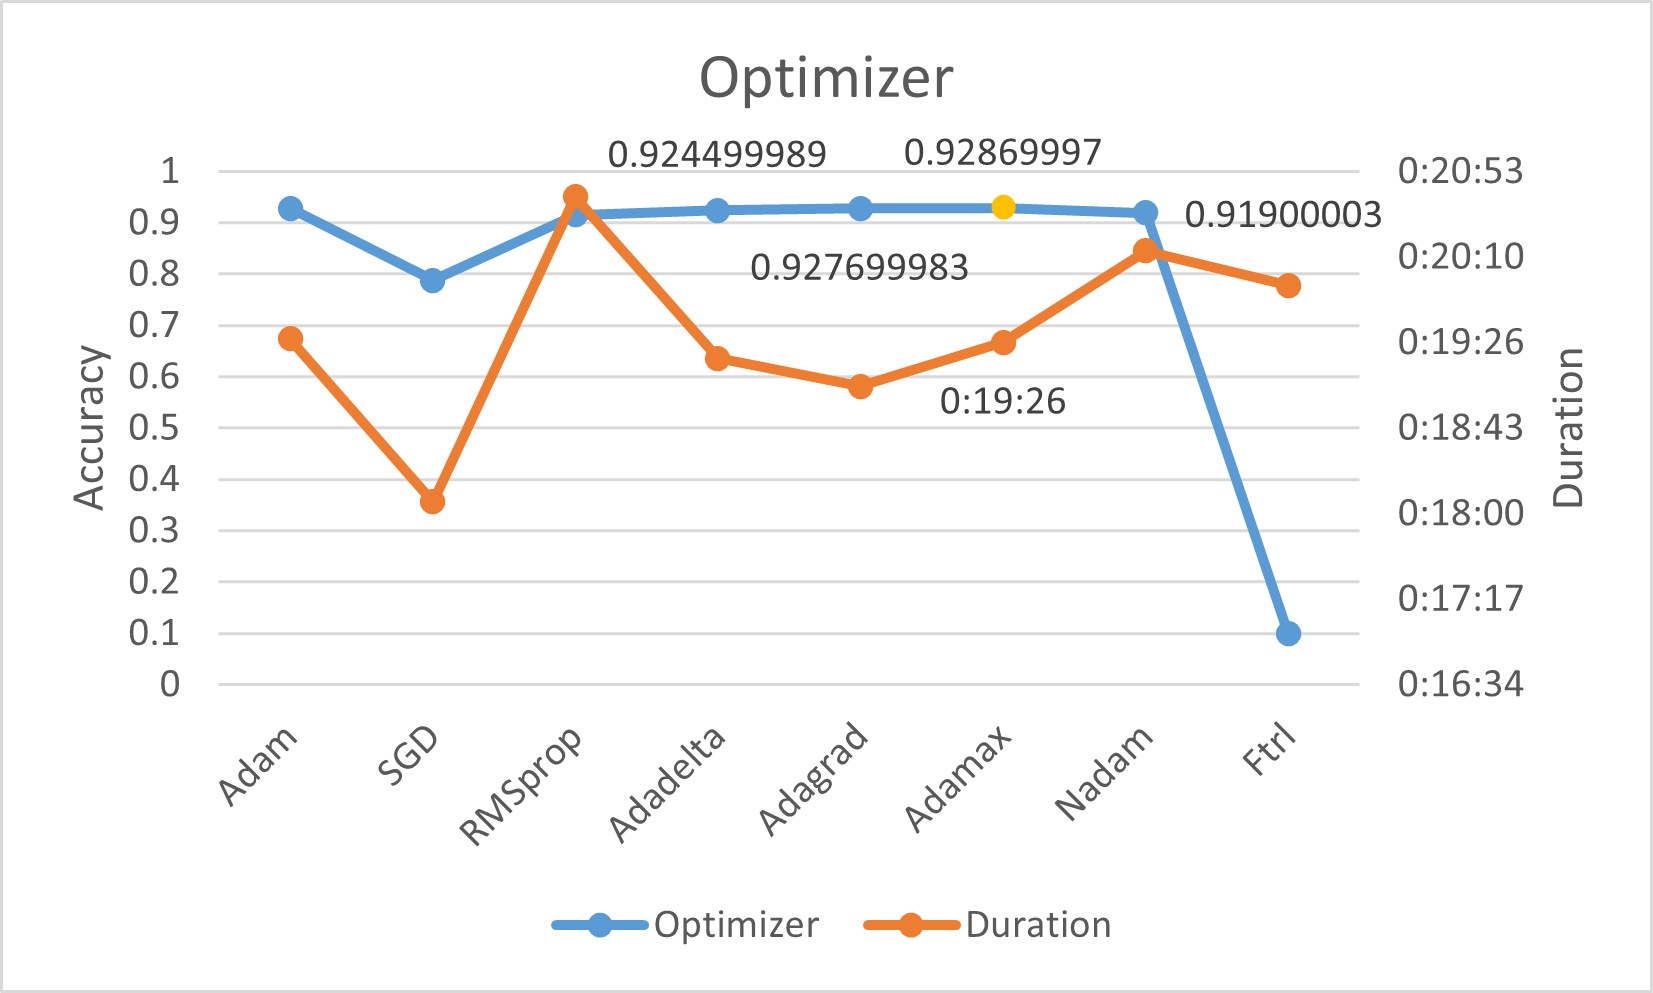
\includegraphics[width=0.7\linewidth]{src/K6}
	\caption{Akurasi dari setiap optimizer yang disediakan oleh keras}
	\label{fig:k6}
\end{figure}
Akurasi tertinggi diperoleh dengan menggunakan optimizer Adamax dengan akurasi mencapai 92.86\%. Setelah mengecek optimizer optimal, langkah berikutnya adalah memilih loss function yang optimal. Loss function yang optimal adalah sparse categorical crossentropy. Hasil eksplorasi disajikan pada gambar \ref{fig:k7} berikut:

% TODO: \usepackage{graphicx} required
\begin{figure}[!h]
	\centering
	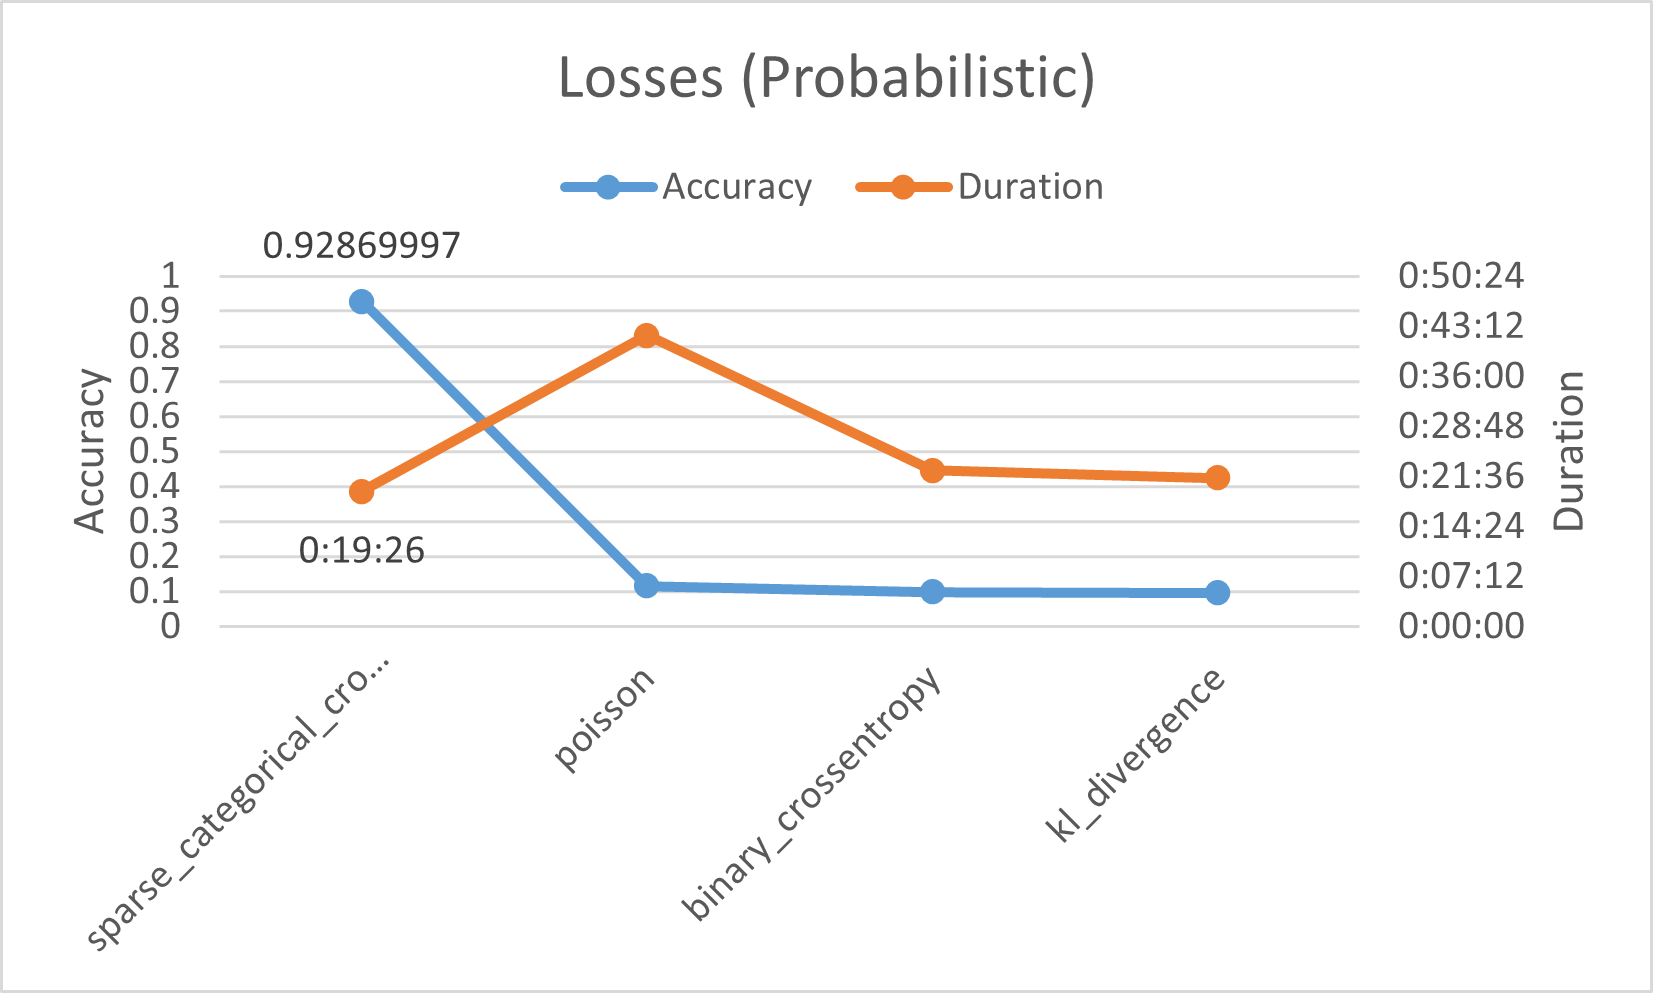
\includegraphics[width=0.7\linewidth]{src/K7}
	\caption{Akurasi dari setiap loss function}
	\label{fig:k7}
\end{figure}

Setelah deperoleh loss function optimal, langkah berikutnya adalah mengeksplorasi model dengan menambahkan learning rate scheduler. Percobaan dilakukan dengan mengkomparasi model tanpa scheduler dengan model dengan scheduler. Percobaan ini menggunakan 10 epoch dan learning rate sebesar $10^{-3}$. Hasil tanpa menggunakan learning rate sceduler mengindikasikan bahwa akurasi pada training test cukup fluktuatif. Hasil eksplorasi tanpa learning rate scheduler disajikan pada gambar \ref{fig:k8} dan pada gambar \ref{fig:k9} disajikan hasil eksplorasi dengan learning rate scheduler.

\begin{figure}[!h]
	\centering
	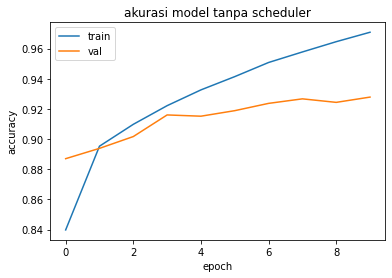
\includegraphics[width=0.7\linewidth]{src/K8.png}
	\caption{Akurasi dari setiap epoch tanpa learning rate scheduler}
	\label{fig:k8}
\end{figure}
\begin{figure}[!h]
	\centering
	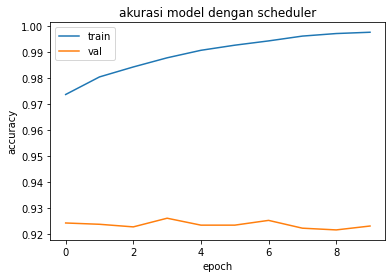
\includegraphics[width=0.7\linewidth]{src/K9.png}
	\caption{Akurasi dari setiap epoch dengan learning rate scheduler}
	\label{fig:k9}
\end{figure}

\subsection{Kesimpulan}
Hasil eksplorasi yang sudah dilakukan menunjukkan bahwa model yang optimal adalah model dengan jumlah kernel pada convolutional layer pertama sebanyak 32 dan jumlah kernel pada convolutional layer kedua sebanyak 128, jumlah dense layer sebanyak 2, jumlah neuron pada setiap dense layer sebanyak 128, optimizer Adamax, loss function sparse categorical crossentropy, dan learning rate scheduler.

\section{Regresi}\label{sec:regresi}


Persoalan regresi yang dilakukan menggunakan data Boston Housing yakni data yang berisi informasi lokasi, kedalaman tanah, dan harga rumah. Setiap catatan dalam dataset Boston Housing menggambarkan kota Boston. Data diambil dari Boston Standard Metropolitan Statistical Area (SMSA) pada tahun 1970. Atributnya didefinisikan sebagai berikut (diambil dari UCI Machine Learning Repository): 
\begin{enumerate}[noitemsep]
	\item CRIM: tingkat kejahatan per kapita menurut kota
	\item ZN: proporsi tanah perumahan yang dikategorikan untuk kavling lebih dari 25.000 sq.ft.
	\item INDUS: proporsi hektar bisnis non-ritel per kota
	\item CHAS: Variabel dummy Sungai Charles (= 1 jika saluran membatasi sungai; 0 sebaliknya)
	\item NOX: konsentrasi oksida nitrat (bagian per 10 juta)
	\item RM: rata-rata jumlah kamar per hunian
	\item AGE: proporsi unit yang ditempati pemilik yang dibangun sebelum 1940
	\item DIS: jarak tertimbang ke lima pusat kerja Boston
	\item RAD: indeks aksesibilitas ke jalan raya radial
	\item TAX: tarif pajak properti nilai penuh per \$10.000
	\item PTRATIO: rasio murid-guru menurut kota
	\item B: 1000(Bk - 0.63)2 di mana Bk adalah proporsi orang kulit hitam menurut kota.
	\item LSTAT: \% status penduduk yang lebih rendah
	\item MEDV: Nilai rata-rata rumah yang ditempati pemilik di \$1000s per kamar.
\end{enumerate}

Percobaan untuk forecasting nilai rata-rata rumah di kota Boston dilakukan dengan menggunakan neural network. Data yang digunakan adalah data training dan data testing. Data training dilakukan dengan menggunakan 80\% data dan data testing dilakukan dengan menggunakan 20\% data. Jumlah epoch yang digunakan sebanyak 200 epoch dan ukuran batch sebanyak 64.

Percebaan pertama dilakukan dengan mengecek jumlah dense layer yang optimal. Percobaan dilakukan dengan membangun model dengan 1 dense layer sampai dengan 5 dense layer. Hasil eksplorasi dari jumlah dense layer optimal adalah jumlah dense layer sebanyak 2. Loss yang dihasilkan sebesar 2.15 dengan menggunakan mean absolute error (MAE) dengan optimizer yang digunakan adalah RMSProp. Hasil eksplorasi dari jumlah dense layer optimal disajikan pada gambar \ref{fig:R1}.    
\begin{figure}[!h]
	\centering
	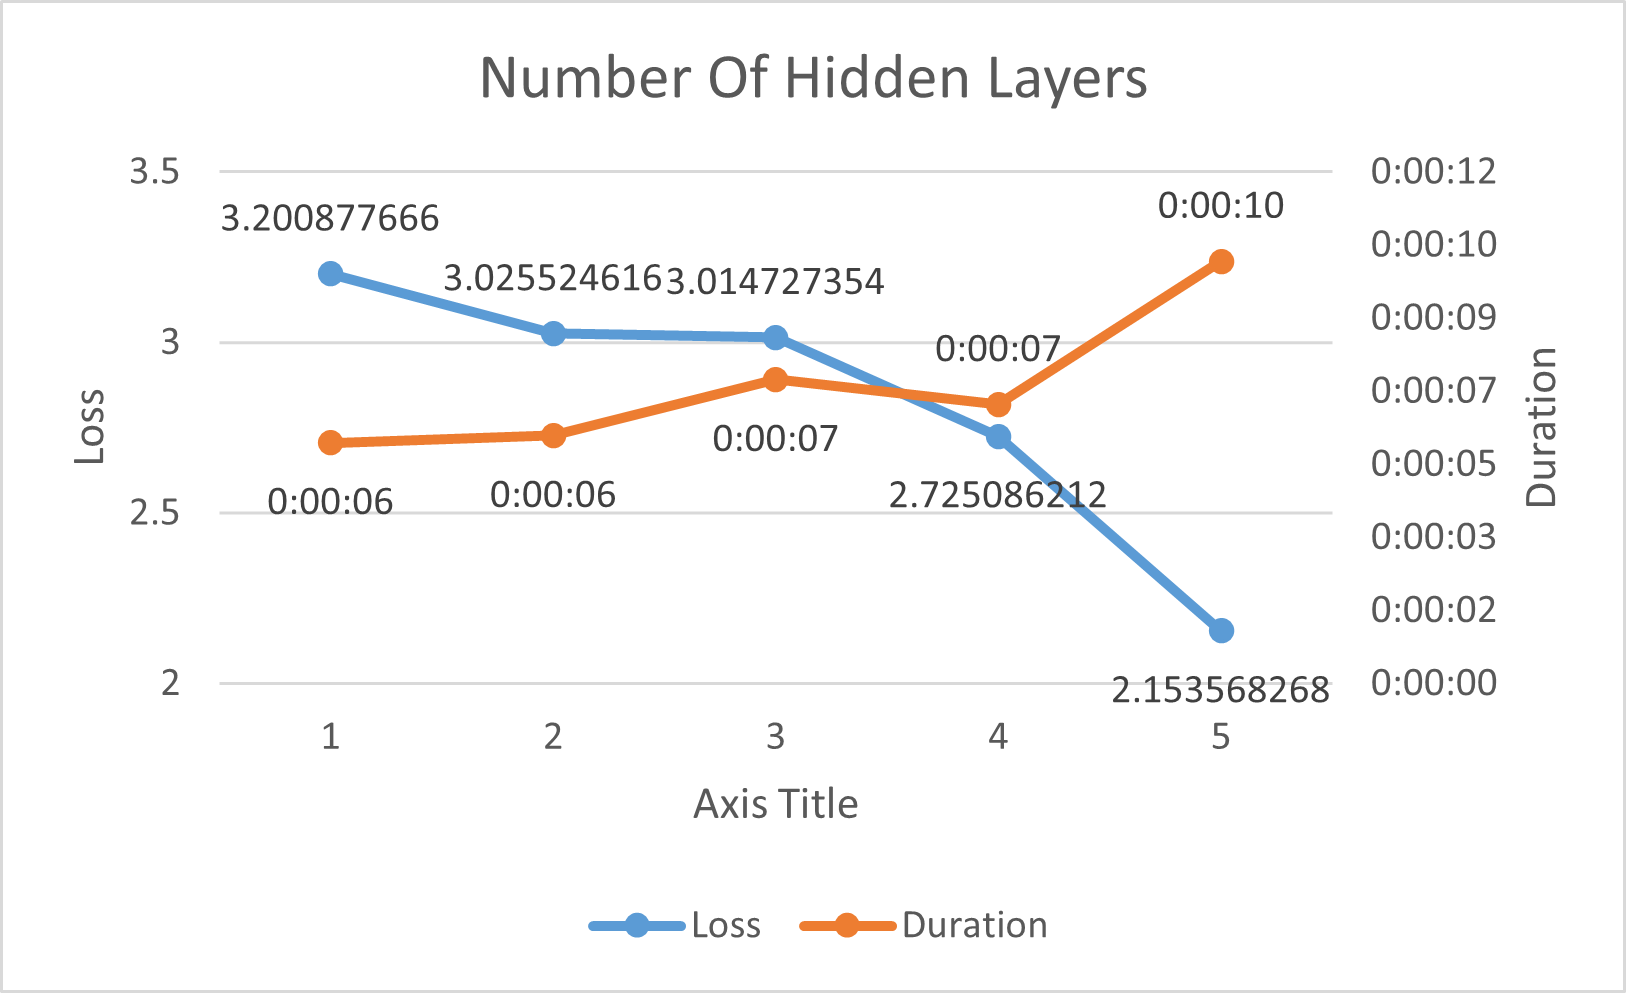
\includegraphics[width=0.7\linewidth]{src/R1}
	\caption{Loss dan MAE dari setiap jumlah dense layer}
	\label{fig:R1}
\end{figure}

Berdasarkan hasil eksplorasi, jumlah dense layer optimal adalah 5 dense layer dengan durasi training sebanyak 200 epoch dan learning rate sebesar $10^{-3}$.
    
Setelah mengecek jumlah dense layer optimal, langkah berikutnya adalah mengecek jumlah neuron optimal pada setiap layer. Percobaan pertama dilakukan dengan melakukan variasi jumlah neuron pada dense layer pertama. Jumlah neuron pada layer kedua sampai kelima dibiarkan tetap sebanyak 128. Percobaan berikutnya dilakukan pada dense layer kedua, ketiga sampai dengan dense layer kelima. Hasil eksplorasi dari jumlah neuron optimal disajikan pada gambar \ref{fig:R2}.


\begin{figure}[!h]
	\centering
	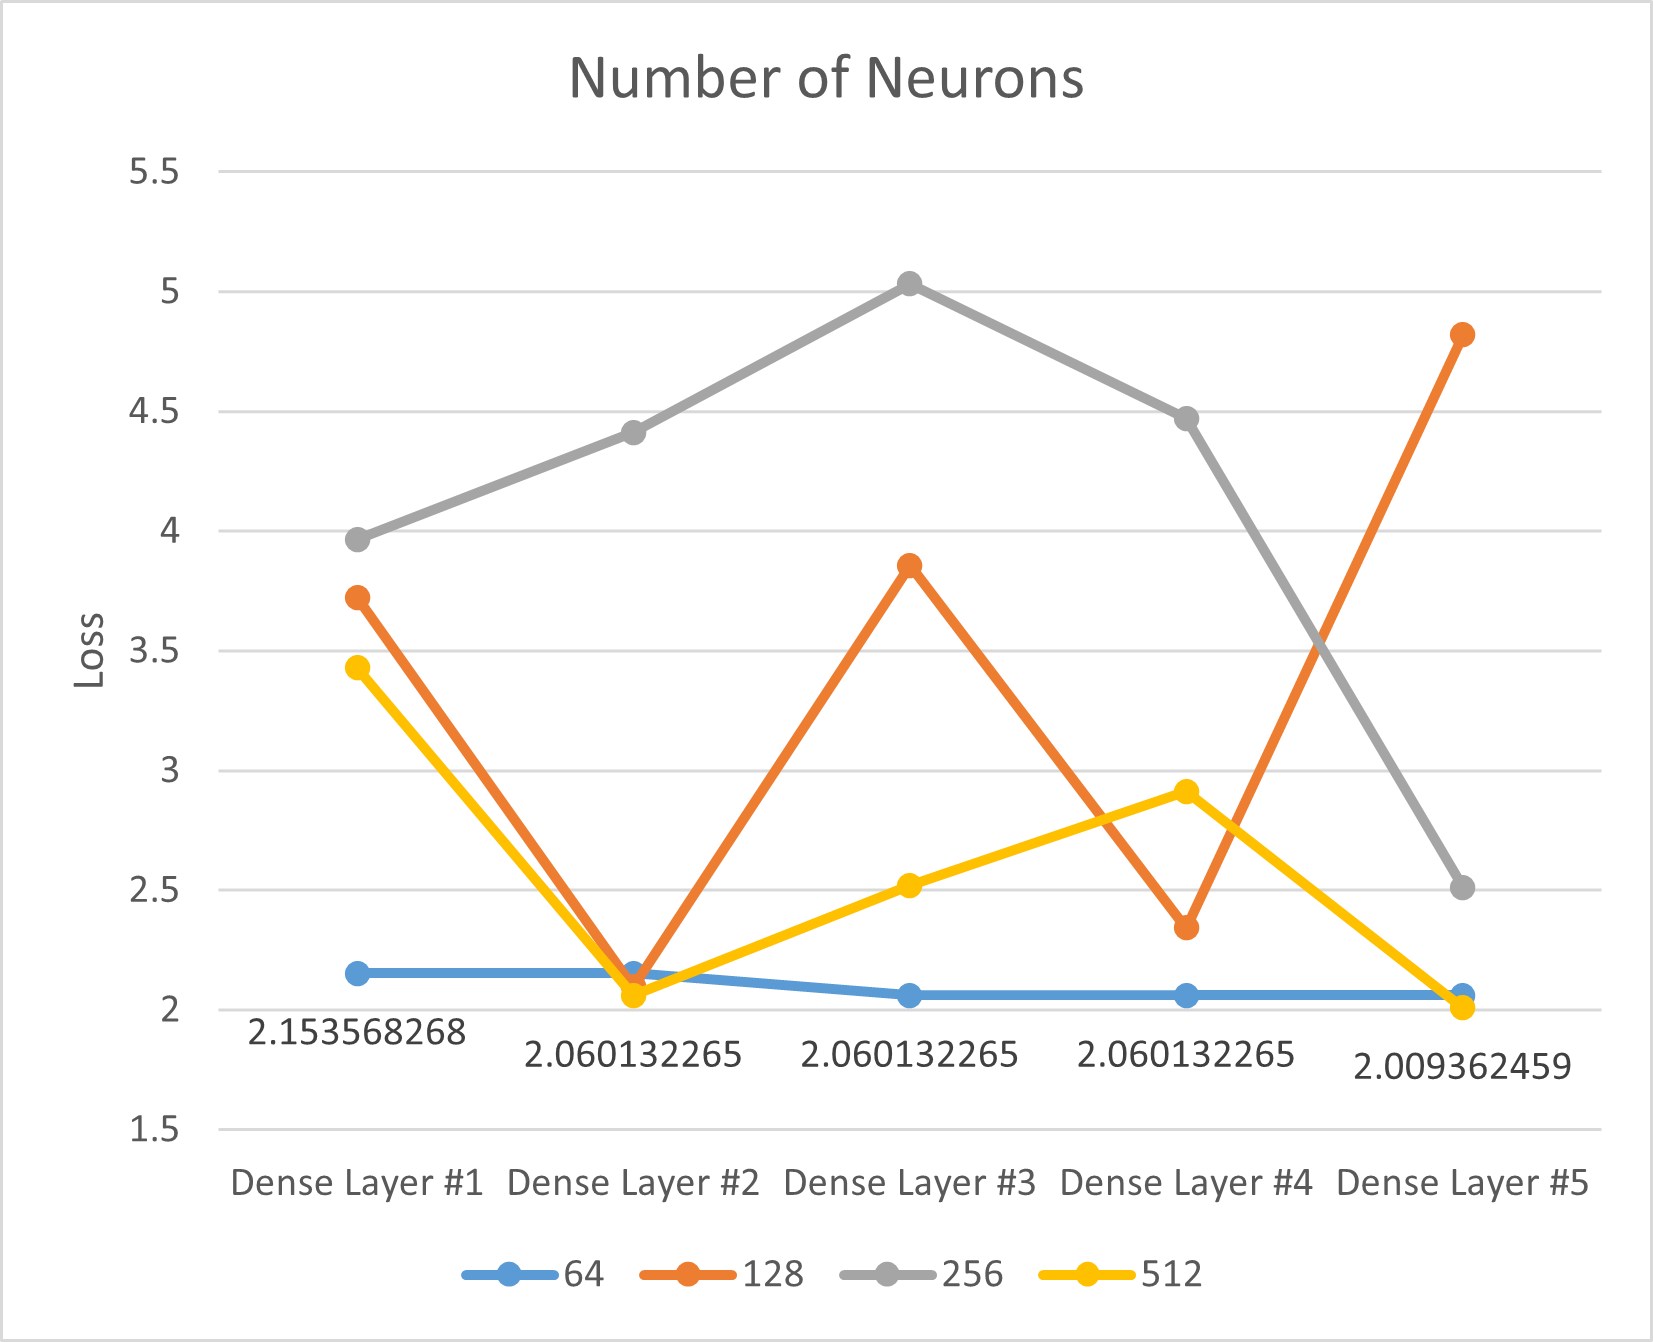
\includegraphics[width=0.7\linewidth]{src/R2}
	\caption{Loss dari setiap percobaan variasi jumlah neuron pada setiap layer}
	\label{fig:R2}
\end{figure}

Hasil eksplorasi yang diperoleh adalah sebagai berikut:
\begin{enumerate}[noitemsep]
	\item Jumlah neuron pada layer pertama optimal adalah 64 neuron.
	\item Jumlah neuron pada layer kedua optimal adalah 512 neuron.
	\item Jumlah neuron pada layer ketiga optimal adalah 64 neuron.
	\item Jumlah neuron pada layer keempat optimal adalah 64 neuron.
	\item Jumlah neuron pada layer kelima optimal adalah 512 neuron.
\end{enumerate}

Setelah mengecek jumlah neuron untuk setiap dense layer, tahap berikutnya adalah mengecek activation function dari setiap dense layer yang optimal. Percobaan pertama dilakukan dengan melakukan variasi activation function pada layer pertama. Percobaan berikutnya dilakukan pada layer kedua, ketiga sampai dengan layer kelima. Hasil eksplorasi dari activation function optimal disajikan pada gambar \ref{fig:R3}.

\begin{figure}[!h]
	\centering
	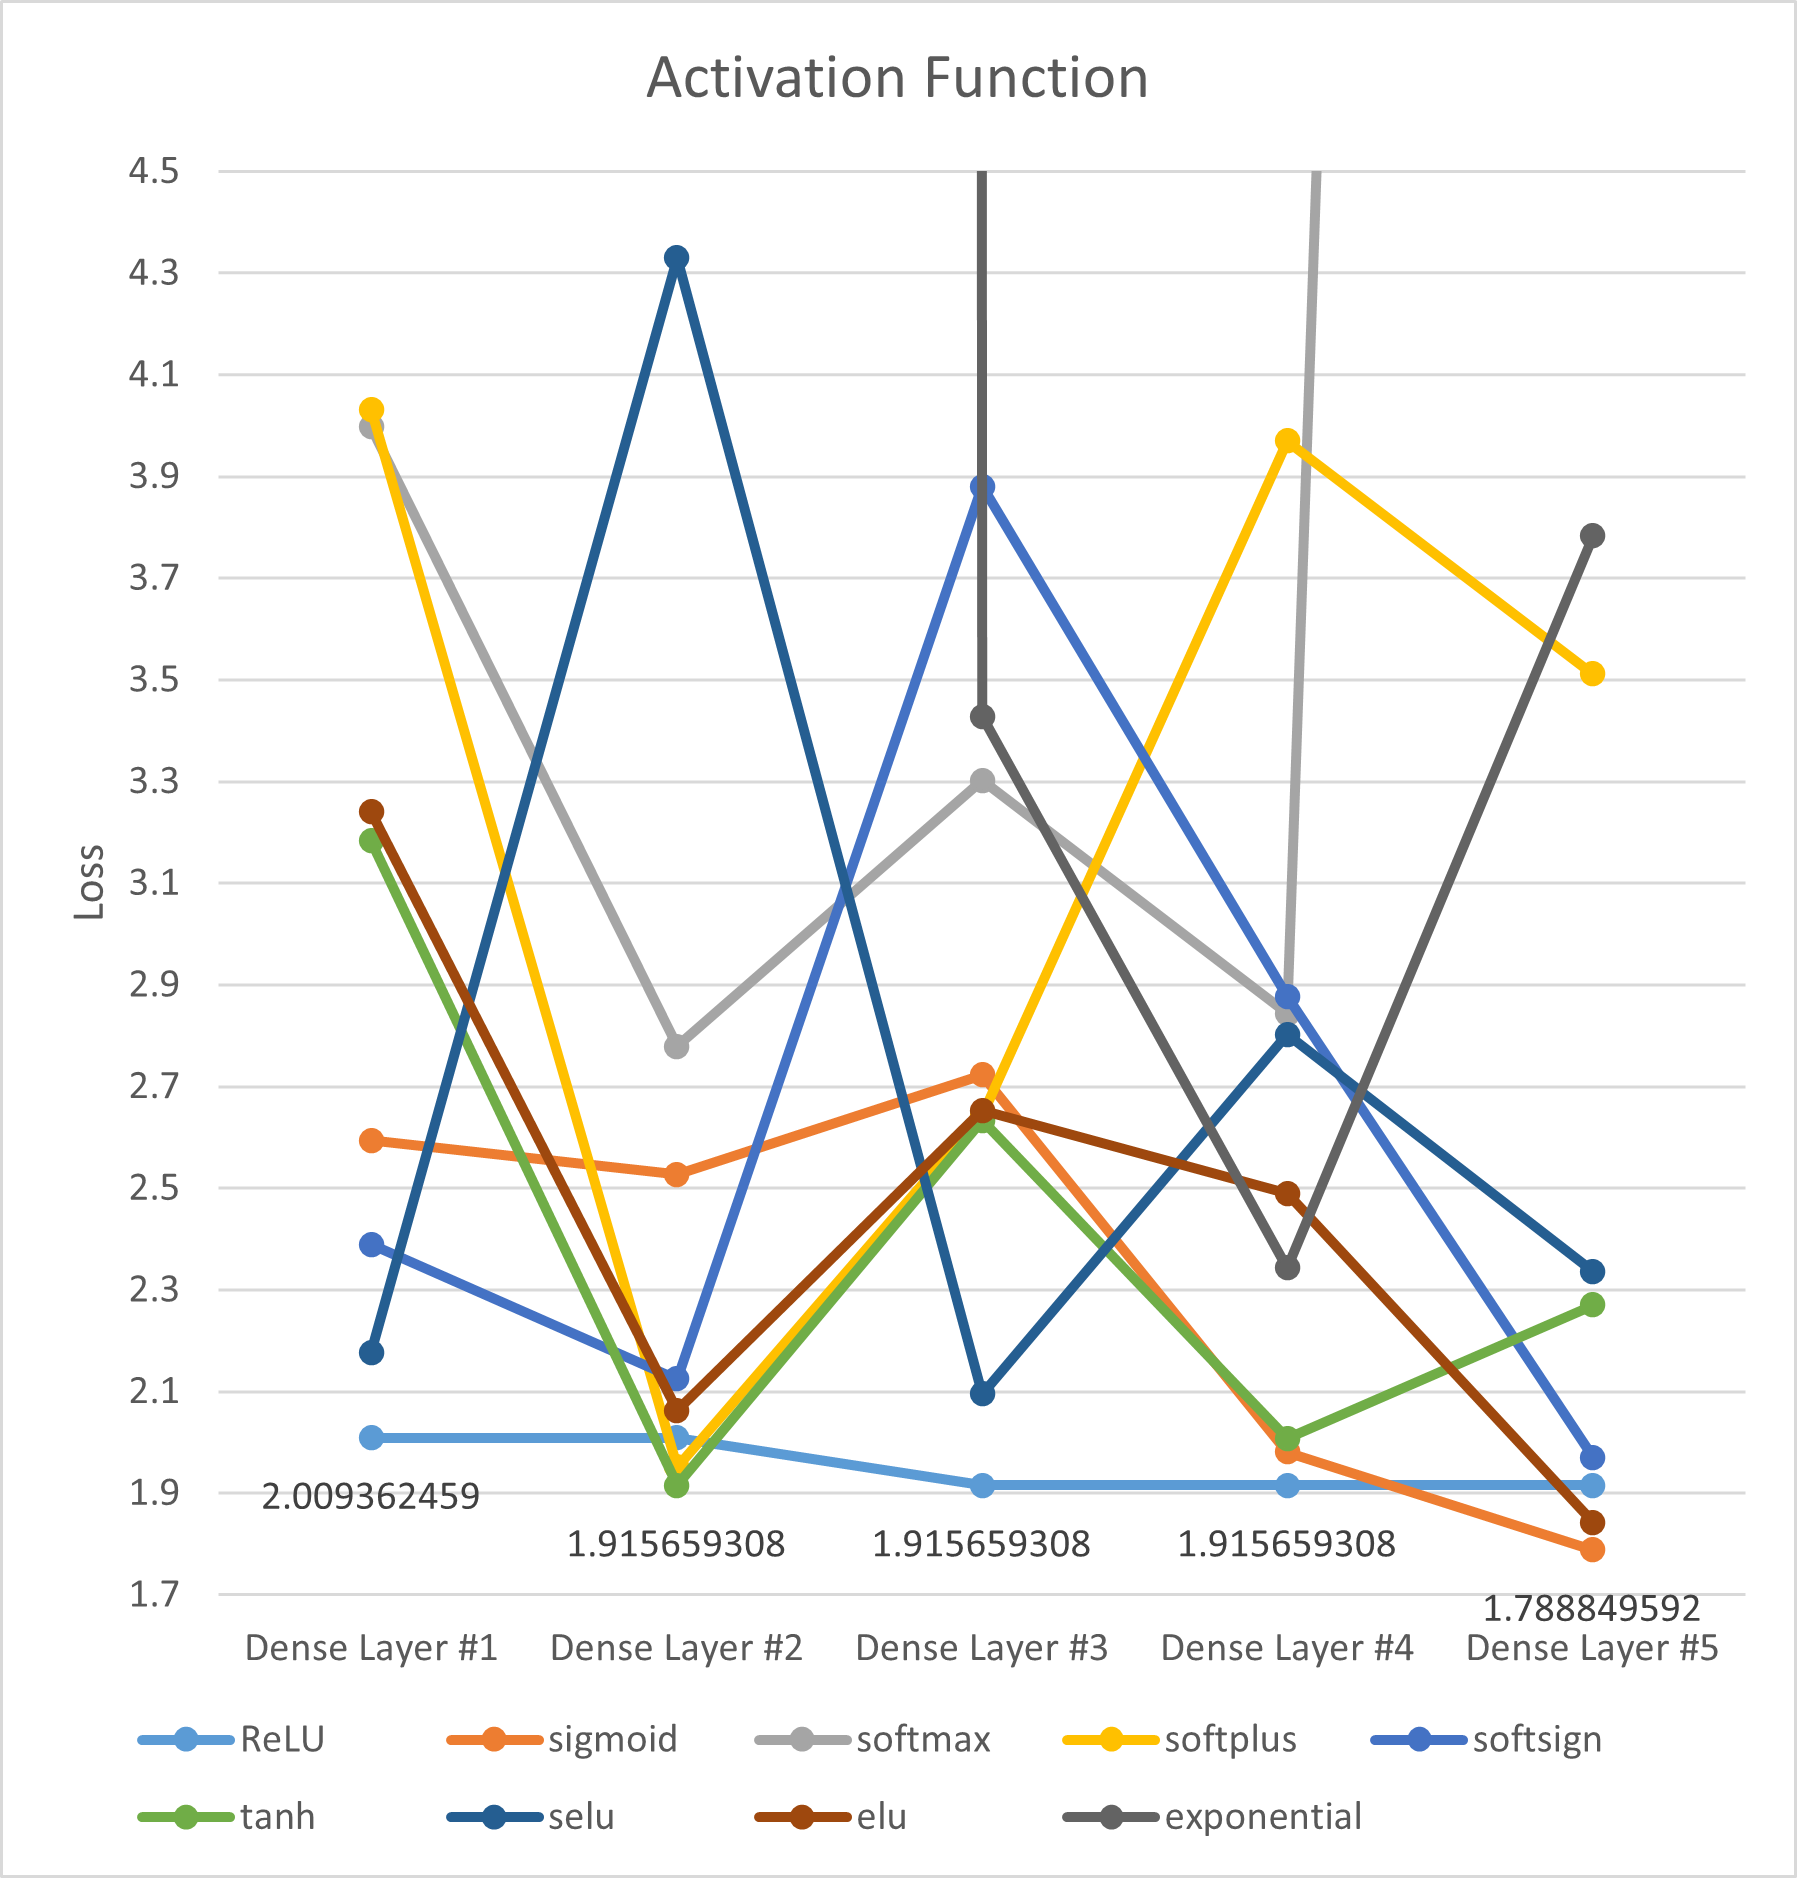
\includegraphics[width=1\linewidth]{src/R3}
	\caption{Loss dari setiap percobaan variasi activation function pada setiap layer}
	\label{fig:R3}
\end{figure}

Hasil eksplorasi yang diperoleh adalah sebagai berikut:
\begin{enumerate}[noitemsep]
	\item Activation function yang optimal pada layer pertama adalah ReLU.
	\item Activation function yang optimal pada layer kedua adalah tanh.
	\item Activation function yang optimal pada layer ketiga adalah ReLU.
	\item Activation function yang optimal pada layer keempat adalah ReLU.
	\item Activation function yang optimal pada layer kelima adalah sigmoid.
\end{enumerate}

Tahap berikutnya adalah mengecek optimizer optimal yang digunakan pada model. Percobaan dilakukan dengan melakukan variasi optimizer pada model. Beberapa optimizer yang diujikan pada model ini adalah Adam, SGD, RMSprop, Adagrad, Adadelta, Adamax, Nadam, TFOptimizer, dan FtrlOptimizer. Hasil eksplorasi dari optimizer optimal disajikan pada gambar \ref{fig:R4}.

\begin{figure}[!h]
	\centering
	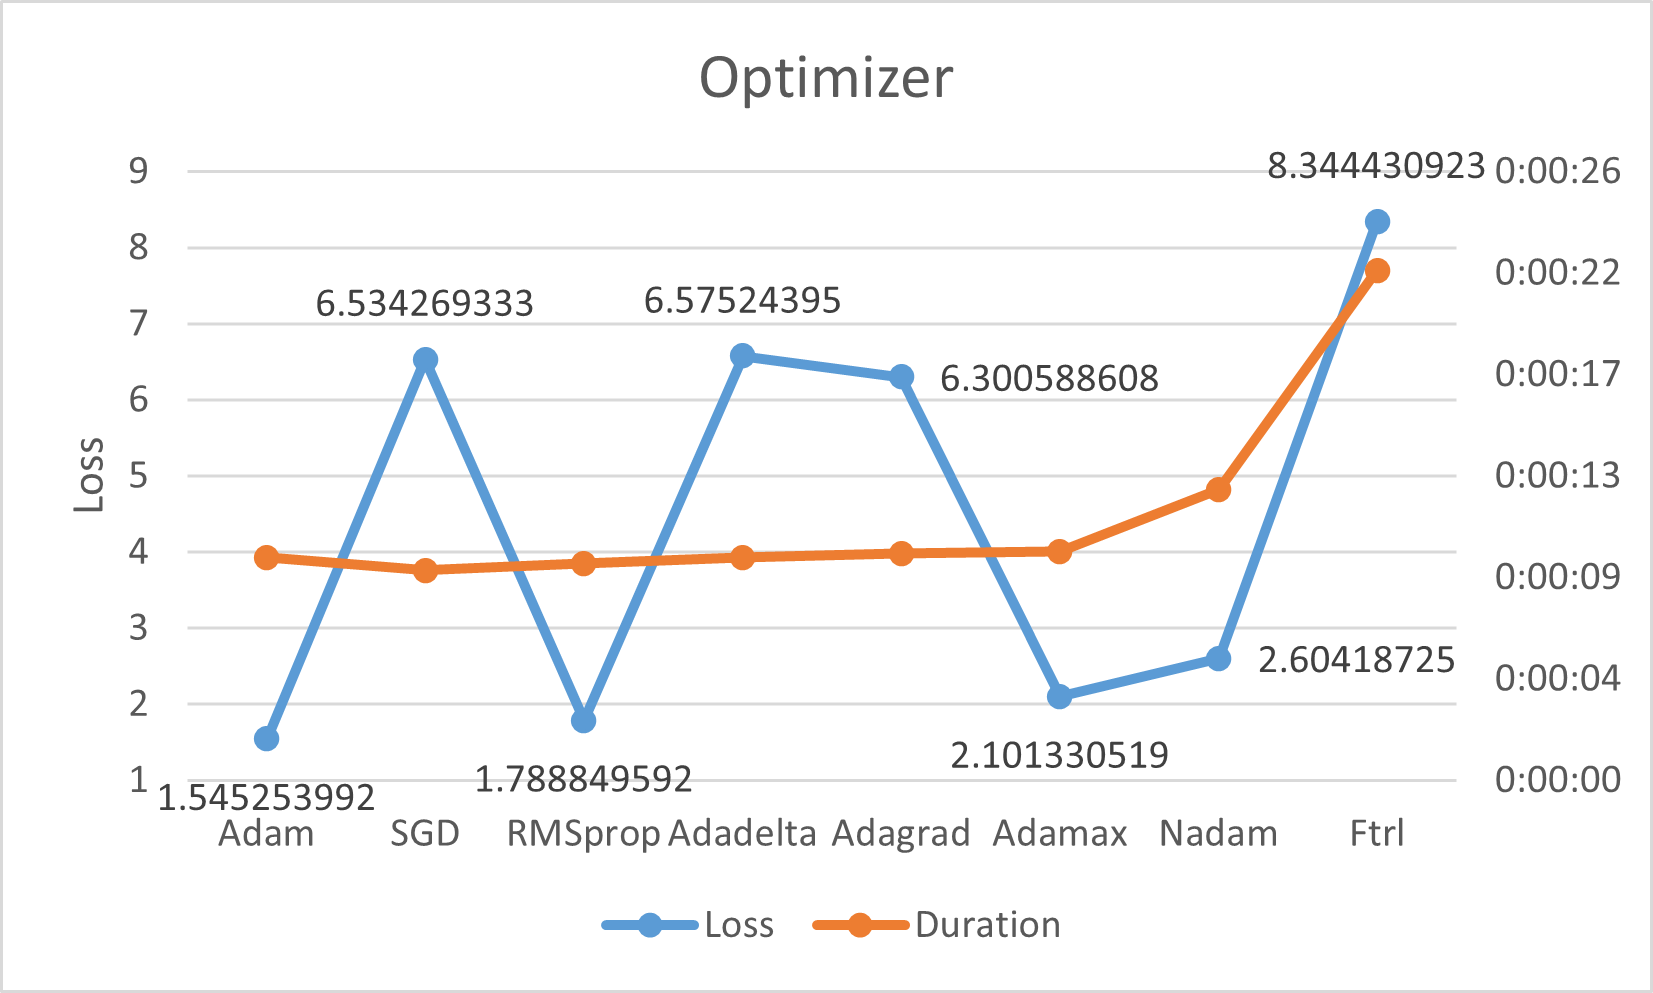
\includegraphics[width=0.7\linewidth]{src/R4}
	\caption{Loss dari setiap percobaan variasi optimizer}
	\label{fig:R4}
\end{figure}

Optimizer terbaik yang diperoleh adalah Adam dengan nilai loss sebesar 1.545.

Setelah mengecek optimizer optimal, tahap berikutnya adalah mengecek loss function optimal yang digunakan pada model. Percobaan dilakukan dengan melakukan variasi loss function pada model. Beberapa loss function yang diujikan pada model ini adalah mean square error (mse), mean absolute error (mae) dan lainnya. Hasil eksplorasi dari learning rate optimal disajikan pada gambar \ref{fig:R5}.

\begin{figure}[!h]
	\centering
	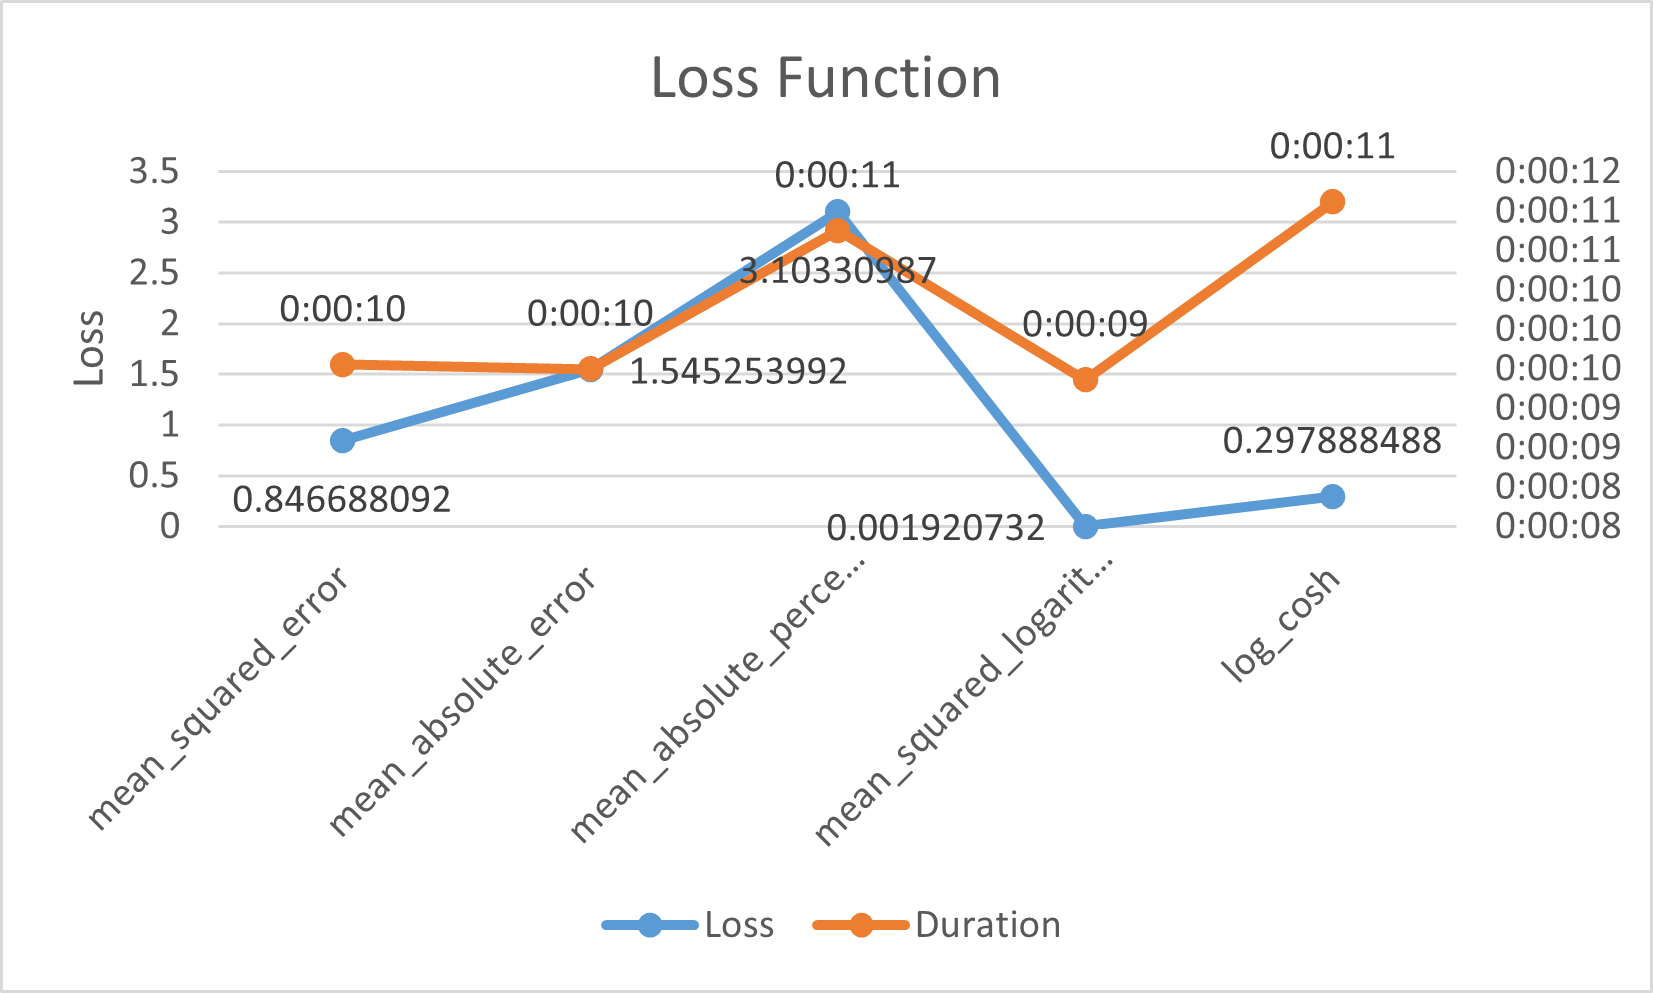
\includegraphics[width=0.7\linewidth]{src/R5}
	\caption{Loss dari setiap percobaan variasi loss function}
	\label{fig:R5}
\end{figure}

Loss funcion terbaik yang diperoleh adalah mean square logaritmic error dengan nilai loss sebesar 0.0019.

\subsection{Kesimpulan}
Kesimpulan dari eksplorasi yang dilakukan adalah sebagai berikut:
\begin{enumerate}[noitemsep]
	\item Jumlah dense layer yang optimal adalah 5 dense layer dengan jumlah neuron pada setiap dense layer adalah 64, 512, 64, 64, dan 512.
	\item Activation function pada setiap dense layer yang optimal adalah ReLU, tanh, ReLU, ReLU, dan sigmoid.
	\item Optimizer yang optimal adalah Adam dengan nilai loss sebesar 1.545.
	\item Loss function yang optimal adalah mean square logaritmic error dengan nilai loss sebesar 0.0019.
\end{enumerate}

% Bibliography
%-----------------------------------------------------------------
%\begin{thebibliography}{99}

%\bibitem{Cd94} Author, \emph{Title}, Journal/Editor, (year)

%\end{thebibliography}

\end{document}
